\clearpage
\begin{explanationbox}
\textbf{\textcolor{CExplanation}{一、从折纸理解：不是同高，而是横纵互换}}
\begin{center}
\begin{minipage}{\linewidth}\centering
\begin{tikzpicture}[x=1.95cm,y=1.95cm,>=stealth,font=\small,line cap=round,line join=round]
\draw[->,gray!75] (-0.35,0)--(3.96,0) node[right=3pt]{$x$};
\draw[->,gray!75] (0,-0.35)--(0,3.96) node[above=3pt]{$y$};
\node at (-.3,.4) {$O$};
\draw[gray,dashed] (-0.15,-0.15)--(3.8,3.8) node[above left=3pt]{$y=x$};

\draw[gray!55,densely dotted] (1,0)--(1,3)--(0,3) (3,0)--(3,1)--(0,1);
\draw[teal,thick] (1,3)--(3,1);
\fill[teal] (1,3) circle(2pt) node[above left=5pt]{$P(1,3)$};
\fill[blue] (3,1) circle(2pt) node[below right=5pt]{$P'(3,1)$};
\fill (2,2) circle(1.8pt) node[right=12pt]{$M(2,2)$};
\draw (1.84,2.16)--(1.68,2)--(1.84,1.84);

\end{tikzpicture}\par\smallskip
{\small $PP^\prime\perp y=x,\qquad PM=MP^\prime$}\par
{\small 中点在镜线上，横纵坐标互换；两轴采用相同单位长度。}\par\smallskip
\end{minipage}
\end{center}


点 $(1,3)$ 折过去是 $(3,1)$，中点 $(2,2)$ 在折线上，连线与 $y=x$ 垂直。与竖直线 $x=a$ 的对称不同，这里横纵坐标都可能改变。折两次回到原点，因此这种交换可以反复使用。
\end{explanationbox}
\clearpage
\begin{explanationbox}
\textbf{\textcolor{CExplanation}{二、指数函数与对数函数}}
\begin{center}
\begin{minipage}{\linewidth}\centering
\begin{tikzpicture}[x=1.35cm,y=1.35cm,>=stealth,font=\small,line cap=round,line join=round]
\draw[->,gray!75] (-3.3,0)--(3.46,0) node[right=3pt]{$x$};
\draw[->,gray!75] (0,-3.3)--(0,3.46) node[above=3pt]{$y$};
\node at (-.3,.4) {$O$};
\draw[gray,dashed] (-3.3,-3.3)--(3.3,3.3) node[above left=3pt]{$y=x$};

\draw[teal,very thick,domain=-3:1.65,samples=120] plot(\x,{2^\x});
\draw[blue,very thick,domain=-3:1.65,samples=120] plot({2^\x},\x);
\draw[orange!80!black,densely dotted] (1,2)--(2,1);
\fill[teal] (0,1) circle(2pt) node[left=4pt]{$(0,1)$};
\fill[blue] (1,0) circle(2pt) node[below right=8pt]{$(1,0)$};
\fill[teal] (1,2) circle(2pt) node[above left=4pt]{$(1,2)$};
\fill[blue] (2,1) circle(2pt) node[below right=4pt]{$(2,1)$};

\end{tikzpicture}\par\smallskip
{\small \textcolor{teal}{\rule[.5ex]{1em}{.8pt}\ $y=2^x$}\qquad\textcolor{blue}{\rule[.5ex]{1em}{.8pt}\ $y=\log_2x$}}\par
{\small 原函数与反函数的对应点交换横纵坐标。}\par\smallskip
\end{minipage}
\end{center}


$y=a^x$（$a>0,a\ne1$）交换横纵坐标得到 $x=a^y$，用对数定义解出 $y=\log_a x$。指数函数定义域为 $\mathbb R$、值域为 $(0,+\infty)$，对数函数恰好相反。点 $(0,1)$ 对应 $(1,0)$，点 $(1,a)$ 对应 $(a,1)$。
\end{explanationbox}
\clearpage
\begin{explanationbox}
\textbf{\textcolor{CExplanation}{三、幂函数：先选单调分支}}
\begin{center}
\begin{minipage}{\linewidth}\centering
\begin{tikzpicture}[x=1.7cm,y=1.7cm,>=stealth,font=\small,line cap=round,line join=round]
\draw[->,gray!75] (-0.35,0)--(4.76,0) node[right=3pt]{$x$};
\draw[->,gray!75] (0,-0.35)--(0,4.76) node[above=3pt]{$y$};
\node at (-.3,.4) {$O$};
\draw[gray,dashed] (-0.15,-0.15)--(4.6,4.6) node[above left=3pt]{$y=x$};

\draw[teal,very thick,domain=0:2,samples=100] plot(\x,{\x*\x});
\draw[blue,very thick,domain=0:2,samples=100] plot({\x*\x},\x);
\draw[orange!80!black,densely dotted] (2,4)--(4,2);
\fill[teal] (2,4) circle(2pt) node[above left=5pt]{$(2,4)$};
\fill[blue] (4,2) circle(2pt) node[below right=5pt]{$(4,2)$};

\end{tikzpicture}\par\smallskip
{\small \textcolor{teal}{\rule[.5ex]{1em}{.8pt}\ $y=x^2,\ x\ge0$}\qquad\textcolor{blue}{\rule[.5ex]{1em}{.8pt}\ $y=\sqrt{x},\ x\ge0$}}\par
{\small 选取非负分支后，每个输出恰好对应一个输入。}\par\smallskip
\end{minipage}
\end{center}


$y=x^2$ 在全体实数上有两个输入 $-2,2$ 对应同一个输出 $4$，折过去会出现 $(4,-2)$ 和 $(4,2)$，不是普通函数。若限制 $x\ge0$，镜像为 $y=\sqrt{x}$；若限制 $x\le0$，镜像为 $y=-\sqrt{x}$。

一般正整数次幂 $x^n$，偶数次幂需要选取一一对应的分支。
\end{explanationbox}
\clearpage
\begin{explanationbox}
\textbf{\textcolor{CExplanation}{三（续）、奇数次幂与奇次方根}}
\begin{center}
\begin{minipage}{\linewidth}\centering
\begin{tikzpicture}[x=1.35cm,y=1.35cm,>=stealth,font=\small,line cap=round,line join=round]
\draw[->,gray!75] (-3.3,0)--(3.46,0) node[right=3pt]{$x$};
\draw[->,gray!75] (0,-3.3)--(0,3.46) node[above=3pt]{$y$};
\node at (-.3,.4) {$O$};
\draw[gray,dashed] (-3.3,-3.3)--(3.3,3.3) node[above left=3pt]{$y=x$};

\draw[teal,very thick,domain=-1.45:1.45,samples=121] plot(\x,{\x^3});
\draw[blue,very thick,domain=-1.45:1.45,samples=121] plot({\x^3},\x);
\fill (1,1) circle(2pt) node[below right=4pt]{$(1,1)$};
\fill (-1,-1) circle(2pt) node[above left=4pt]{$(-1,-1)$};

\end{tikzpicture}\par\smallskip
{\small \textcolor{teal}{\rule[.5ex]{1em}{.8pt}\ $y=x^3$}\qquad\textcolor{blue}{\rule[.5ex]{1em}{.8pt}\ $y=\sqrt[3]{x}$}}\par
{\small 两函数的定义域、值域均为实数集，无须截取分支。}\par\smallskip
\end{minipage}
\end{center}


立方函数 $y=x^3$ 在全体实数上严格递增，镜像为 $y=\sqrt[3]{x}$，无须截半。一般正奇数次幂可用全体实数作为定义域。
\end{explanationbox}
\clearpage
\begin{explanationbox}
\textbf{\textcolor{CExplanation}{四、三角函数与反三角函数}}
\begin{center}
\begin{minipage}{\linewidth}\centering
\begin{tikzpicture}[x=1.7cm,y=1.7cm,>=stealth,font=\small,line cap=round,line join=round]
\draw[->,gray!75] (-2.3,0)--(2.46,0) node[right=3pt]{$x$};
\draw[->,gray!75] (0,-2.3)--(0,2.46) node[above=3pt]{$y$};
\node at (-.3,.4) {$O$};
\draw[gray,dashed] (-2.3,-2.3)--(2.3,2.3) node[above left=3pt]{$y=x$};

\draw[teal,very thick,domain=-pi/2:pi/2,samples=121] plot(\x,{sin(\x r)});
\draw[blue,very thick,domain=-pi/2:pi/2,samples=121] plot({sin(\x r)},\x);
\fill[teal] ({pi/2},1) circle(2pt) node[right=5pt]{$(\pi/2,1)$};
\fill[blue] (1,{pi/2}) circle(2pt) node[above=5pt]{$(1,\pi/2)$};
\fill[teal] ({-pi/2},-1) circle(2pt) node[left=5pt]{$(-\pi/2,-1)$};
\fill[blue] (-1,{-pi/2}) circle(2pt) node[below=5pt]{$(-1,-\pi/2)$};

\end{tikzpicture}\par\smallskip
{\small \textcolor{teal}{\rule[.5ex]{1em}{.8pt}\ $y=\sin x,\ |x|\le\pi/2$}\qquad\textcolor{blue}{\rule[.5ex]{1em}{.8pt}\ $y=\arcsin x,\ |x|\le1$}}\par
{\small 实心端点互为镜像，两个闭区间的角色交换。}\par\smallskip
\end{minipage}
\end{center}


三角函数须限制到标准单调区间才得到通常的反三角函数：
\begin{center}\renewcommand{\arraystretch}{1.5}
\begin{tabular}{c|c|c}
原函数 & 原函数定义域 & 反函数\\\hline
$\sin x$ & $[-\pi/2,\pi/2]$ & $\arcsin x$\\
$\cos x$ & $[0,\pi]$ & $\arccos x$\\
$\tan x$ & $(-\pi/2,\pi/2)$ & $\arctan x$
\end{tabular}\end{center}
前两个反函数定义域为 $[-1,1]$，第三个为 $\mathbb R$。反三角函数作为拓展理解，不要求所有高中课程都系统学习。
\end{explanationbox}
\clearpage
\begin{explanationbox}
\textbf{\textcolor{CExplanation}{五、一次函数与自身对称的模型}}
\begin{center}
\begin{minipage}{\linewidth}\centering
\begin{tikzpicture}[x=1.35cm,y=1.35cm,>=stealth,font=\small,line cap=round,line join=round]
\draw[->,gray!75] (-3.3,0)--(3.46,0) node[right=3pt]{$x$};
\draw[->,gray!75] (0,-3.3)--(0,3.46) node[above=3pt]{$y$};
\node at (-.3,.4) {$O$};
\draw[gray,dashed] (-3.3,-3.3)--(3.3,3.3) node[above left=3pt]{$y=x$};

\foreach \s in {-1,1}{\draw[teal,very thick,domain=.333333:3,samples=120] plot({\s*\x},{\s/\x});}
\draw[orange!80!black,densely dotted,thick] (2,.5)--(.5,2);
\fill[teal] (2,.5) circle(2pt) node[above right=6pt]{$(2,1/2)$};
\fill[teal] (.5,2) circle(2pt) node[above right=6pt]{$(1/2,2)$};

\end{tikzpicture}\par\smallskip
{\small \textcolor{teal}{$y=1/x\ (x\ne0)$：原函数与反函数图象完全重合}}\par
{\small 交换坐标后仍满足 $xy=1$；两条分支都必须保留。}\par\smallskip
\end{minipage}
\end{center}


$y=kx+b$（$k\ne0$）交换得 $x=ky+b$，所以反函数是 $y=(x-b)/k$。若要求原直线和镜像完全相同，则 $k=1,b=0$ 或 $k=-1$、$b$ 任意。

$y=k/x$ 也可写作 $xy=k$，交换后完全不变。若把它沿 $y=x$ 方向平移到 $(a,a)$，得到 $(x-a)(y-a)=k$，仍然不变，即 $y=a+k/(x-a)$。
\end{explanationbox}
\clearpage
\begin{explanationbox}
\textbf{\textcolor{CExplanation}{六、圆、椭圆与圆锥曲线的统一变换}}
\begin{center}
\begin{minipage}{\linewidth}\centering
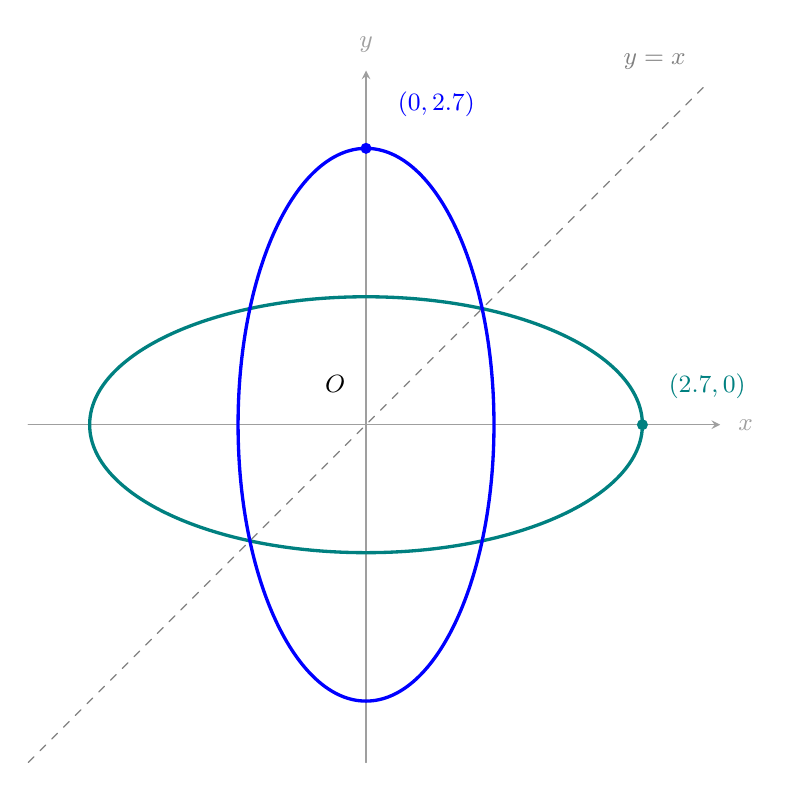
\begin{tikzpicture}[x=1.3cm,y=1.3cm,>=stealth,font=\small,line cap=round,line join=round]
\draw[->,gray!75] (-3.3,0)--(3.46,0) node[right=3pt]{$x$};
\draw[->,gray!75] (0,-3.3)--(0,3.46) node[above=3pt]{$y$};
\node at (-.3,.4) {$O$};
\draw[gray,dashed] (-3.3,-3.3)--(3.3,3.3) node[above left=3pt]{$y=x$};

\draw[teal,very thick] (0,0) ellipse (2.7 and 1.25);
\draw[blue,very thick] (0,0) ellipse (1.25 and 2.7);
\fill[teal] (2.7,0) circle(2pt) node[above right=6pt]{$(2.7,0)$};
\fill[blue] (0,2.7) circle(2pt) node[above right=8pt]{$(0,2.7)$};

\end{tikzpicture}\par\smallskip
{\small \textcolor{teal}{\rule[.5ex]{1em}{.8pt}\ $x^2/2.7^2+y^2/1.25^2=1$}\qquad\textcolor{blue}{\rule[.5ex]{1em}{.8pt}\ $y^2/2.7^2+x^2/1.25^2=1$}}\par
{\small 椭圆的长、短轴交换，半轴长度不变。}\par\smallskip
\end{minipage}
\end{center}


\begin{itemize}[leftmargin=*,itemsep=.4em]
\item 圆 $(x-a)^2+(y-b)^2=r^2$ 的镜像圆心为 $(b,a)$，半径不变；当 $a=b$ 时自身对称。
\item 椭圆 $x^2/a^2+y^2/b^2=1$ 镜像为 $y^2/a^2+x^2/b^2=1$。
\item 抛物线 $y^2=2px$ 镜像为 $x^2=2py$。
\item 双曲线 $x^2/a^2-y^2/b^2=1$ 镜像为 $y^2/a^2-x^2/b^2=1$。
\end{itemize}
图中先单独展示椭圆的反射。曲线不必是函数，仍可直接交换坐标。
\end{explanationbox}
\clearpage
\begin{explanationbox}
\textbf{\textcolor{CExplanation}{六（续）、抛物线的反射}}
\begin{center}
\begin{minipage}{\linewidth}\centering
\begin{tikzpicture}[x=1.35cm,y=1.35cm,>=stealth,font=\small,line cap=round,line join=round]
\draw[->,gray!75] (-3.3,0)--(3.46,0) node[right=3pt]{$x$};
\draw[->,gray!75] (0,-3.3)--(0,3.46) node[above=3pt]{$y$};
\node at (-.3,.4) {$O$};
\draw[gray,dashed] (-3.3,-3.3)--(3.3,3.3) node[above left=3pt]{$y=x$};

\draw[teal,very thick,domain=-3:3,samples=121] plot({\x*\x/4},\x);
\draw[blue,very thick,domain=-3:3,samples=121] plot(\x,{\x*\x/4});
\draw[orange!80!black,densely dotted] (1,2)--(2,1);
\fill[teal] (1,2) circle(2pt) node[left=5pt]{$(1,2)$};
\fill[blue] (2,1) circle(2pt) node[below right=8pt]{$(2,1)$};
\draw[teal,dashed] (.3,1.3)--(1.7,2.7);
\draw[blue,dashed] (1.3,.3)--(2.7,1.7);

\end{tikzpicture}\par\smallskip
{\small \textcolor{teal}{\rule[.5ex]{1em}{.8pt}\ $y^2=4x$}\qquad\textcolor{blue}{\rule[.5ex]{1em}{.8pt}\ $x^2=4y$}}\par
{\small 对应切点 $(1,2)$ 与 $(2,1)$ 处，切线斜率均为 $1$。}\par\smallskip
\end{minipage}
\end{center}


横向抛物线 $y^2=4x$ 交换坐标后成为竖向抛物线 $x^2=4y$；图中的对应点及切线也随之反射。
\end{explanationbox}
\clearpage
\begin{explanationbox}
\textbf{\textcolor{CExplanation}{七、斜率与交点为什么容易考}}
\begin{center}
\begin{minipage}{\linewidth}\centering
\begin{tikzpicture}[x=1.35cm,y=1.35cm,>=stealth,font=\small,line cap=round,line join=round]
\draw[->,gray!75] (-3.3,0)--(3.46,0) node[right=3pt]{$x$};
\draw[->,gray!75] (0,-3.3)--(0,3.46) node[above=3pt]{$y$};
\node at (-.3,.4) {$O$};
\draw[gray,dashed] (-3.3,-3.3)--(3.3,3.3) node[above left=3pt]{$y=x$};

\draw[teal,very thick] (-1.5,-3)--(1.5,3);
\draw[blue,very thick] (-3,-1.5)--(3,1.5);
\draw[teal,densely dotted,thick] (0,0)--(1,0)--(1,2);
\draw[blue,densely dotted,thick] (0,0)--(0,1)--(2,1);
\node[teal,below=5pt] at (.5,0) {$1$};
\node[teal] at (1.4,1.9) {$2$};
\node[blue,left=5pt] at (-.2,.8) {$1$};
\node[blue] at (1.75,1.35) {$2$};
\fill[teal] (1,2) circle(2pt);
\fill[blue] (2,1) circle(2pt);

\end{tikzpicture}\par\smallskip
{\small \textcolor{teal}{\rule[.5ex]{1em}{.8pt}\ $y=2x,\ k=2/1=2$}\qquad\textcolor{blue}{\rule[.5ex]{1em}{.8pt}\ $y=x/2,\ k^\prime=1/2$}}\par
{\small 横纵增量互换，斜率互为倒数，符号保持不变。}\par\smallskip
\end{minipage}
\end{center}


一条线沿横方向走 $\Delta x$、纵方向走 $\Delta y$，镜像之后两者互换，斜率就从 $\Delta y/\Delta x$ 变成 $\Delta x/\Delta y$。不要把镜像误认为垂直。

若递增函数存在一对 $a<b$ 且 $f(a)=b,f(b)=a$，递增性会要求 $b<a$，矛盾。因此递增函数的交点必须在镜线上；递减函数却允许这种交换。
\end{explanationbox}
